\chapter{Appendix}
\label{app2}

\section{State Transition Diagram in eXpOS}

\begin{figure}[ht]
\centering
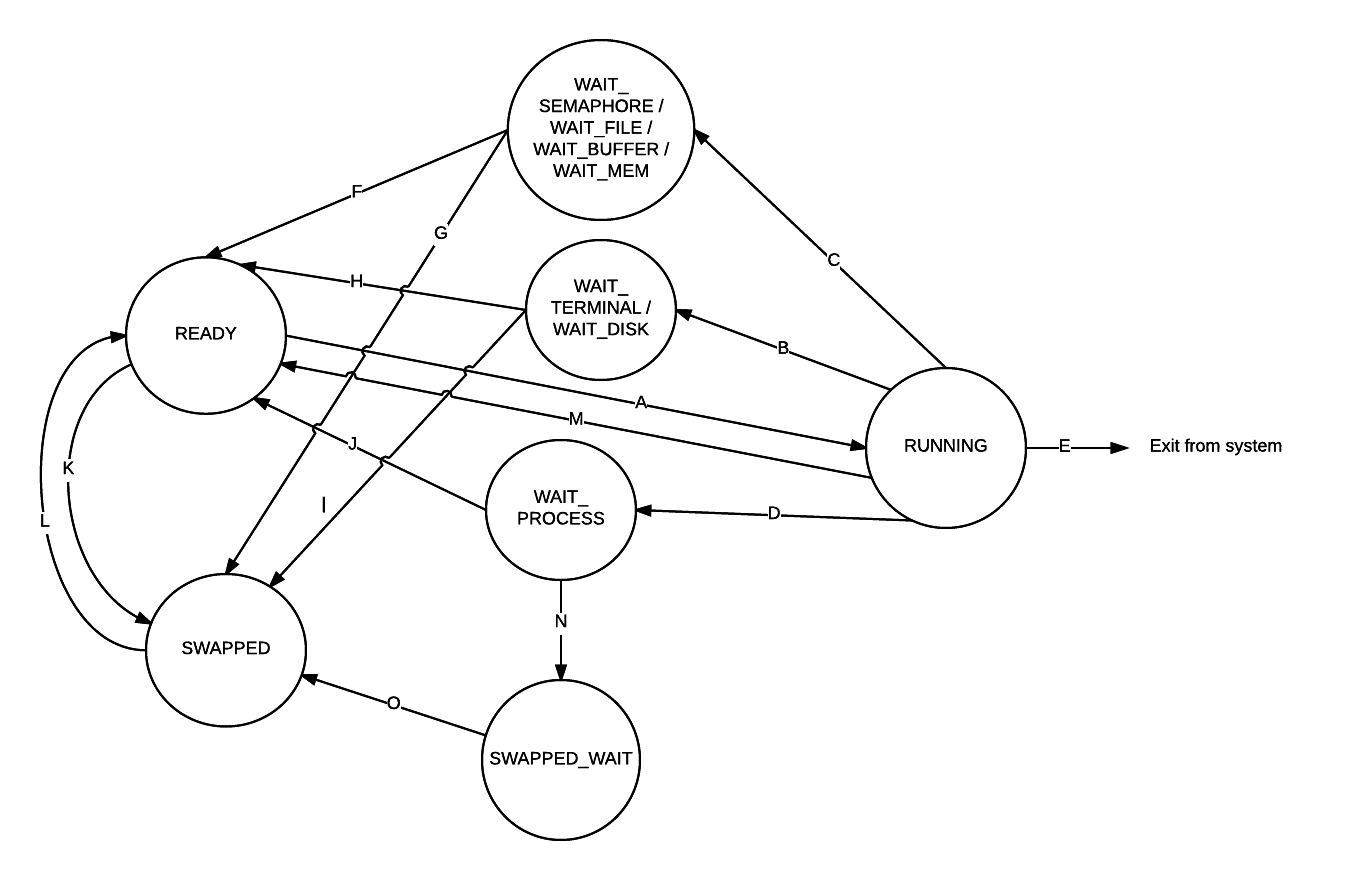
\includegraphics[scale=0.70]{figures/state.png}
\caption{\footnotesize State Transitions}
\label{fig_1}
\end{figure}

\textbf{A}\\
READY $\rightarrow$ RUNNING : The scheduler has scheduled the process for execution.

\textbf{B}\\
RUNNING  $\rightarrow$ WAIT\_TERMINAL : The process is either waiting for access to the terminal or for data to be inputted through terminal.\\
RUNNING  $\rightarrow$ WAIT\_DISK :  The process is either waiting for access to the disk or for the disk operation to finish.

\textbf{C}\\
RUNNING $\rightarrow$ WAIT\_SEMAPHORE : The semaphore which the process is trying to use, is found to be locked.\\
RUNNING $\rightarrow$ WAIT\_FILE : The file which the process is trying to read/write, is found to be locked.\\
RUNNING $\rightarrow$ WAIT\_BUFFER : The buffer which the process is trying to use, is found to be locked.\\
RUNNING $\rightarrow$ WAIT\_MEM : The process requires a free memory page but there are none in the memory.

\textbf{D}\\
RUNNING $\rightarrow$ WAIT\_PROCESS : The process is waiting for another process to either exit or to signal it.

\textbf{E}\\
RUNNING $\rightarrow$ Exit from system : The process has either completed execution or has invoked an Exit System Call.

\textbf{F}\\
WAIT\_SEMAPHORE $\rightarrow$ READY : The semaphore for which the process was waiting, is now unlocked.\\
WAIT\_FILE $\rightarrow$ READY : The file for which the process was waiting, is now unlocked.\\
WAIT\_BUFFER $\rightarrow$ READY : The buffer for which the process was waiting, is now unlocked.\\
WAIT\_MEM $\rightarrow$ READY : There are free pages in memory.\\

\textbf{G}\\
WAIT\_SEMAPHORE / WAIT\_FILE / WAIT\_BUFFER / WAIT\_MEM $\rightarrow$ SWAPPED : The current stack page of the process has been swapped out.

\textbf{H}\\
WAIT\_TERMINAL $\rightarrow$ READY : The input data has been read from terminal and terminal is free to be used by any process.\\
WAIT\_DISK $\rightarrow$ READY : The disk operation is complete.


\textbf{I}\\
WAIT\_TERMINAL / WAIT\_DISK $\rightarrow$ SWAPPED : The current stack page of the process has been swapped out.

\textbf{J}\\
WAIT\_PROCESS $\rightarrow$ READY : The process has either received a signal from the process it was waiting for or the latter has exited the system.

\textbf{K}\\
READY $\rightarrow$ SWAPPED : The current stack page of the process has been swapped out.

\textbf{L}\\
SWAPPED $\rightarrow$ READY : The stack page required by the process to continue execution was swapped in.

\textbf{M}\\
RUNNING $\rightarrow$ READY : Context switch caused by the timer interrupt routine.

\textbf{N}\\
WAIT\_PROCESS $\rightarrow$ SWAPPED\_WAIT : The current stack page of the process was swapped out while waiting for another process.

\textbf{O}\\
SWAPPED\_WAIT $\rightarrow$ SWAPPED : The process in SWAPPED\_WAIT state has either received a signal from the process it was waiting for or the latter has exited.


